\chapter{Positionsbestimmung}\label{kapitel-2}

Dieses Kapitel behandelt die Frage, wie es autonome Fahrzeuge schaffen, sich selbst in unterschiedlichsten Verkehrssituationen auf wenige \si{\centi\meter} genau zu lokalisieren. Gerade im Verkehr ist eine besonders hohe Genauigkeit gefragt, eine ungefähre Standortbestimmung ist für autonome Fahrzeuge definitiv nicht ausreichend.


\section{Satellitenortung}

Das wohl bekannteste heute eingesetzte Ortungssystem, welches auf Satellitenortung basiert, ist das \ac{GPS}, welches vom US-Verteidigungsministerium betrieben wird. \vgl{Hilty} In etwa \SI{20000}{\kilo\meter} Höhe umkreisen 31 Satelliten zweimal täglich die Erde und senden Funksignale auf aus, welche Informationen zu Position und Uhrzeit des Satelliten enthalten. Die Genauigkeit bei einer \ac{GPS}-Ortung liegt bei ungefähr 5 \si{\meter}.
\vgl{Winner}

Das russische GLONASS und das europäische Galileo-Projekt sind zwei weitere satellitenbasierte Ortungssysteme. Ein wichtiger Vorteil dieser beiden Systeme liegt darin, dass in Kombination mit \ac{GPS} und damit verbunden einer größeren Satellitenzahl, eine höhere Genauigkeit und Zuverlässigkeit der Ortung erreichbar ist.
\vgl{Hilty}

\subsection{Berechnung des Standortes}

Die Positionsbestimmung erfolgt bei \ac{GPS} durch Entfernungsmessung zu mehreren Satelliten. Ein Satellit ist nicht ausreichend, da sich der Empfänger überall auf der Oberfläche einer Kugel befinden kann, deren Mittelpunkt der Standort des Satelliten und Radius die Entfernung zwischen Sender und Empfänger ist. Um alle drei Koordinaten (x, y, z) berechnen zu können, sind Entfernungen zu drei Satelliten notwending, um die erforderlichen Gleichungen aufstellen zu können.

Die Entfernungsmessung geschieht durch Messung der Laufzeit des Signals (\dH die Zeit, die das Signal für die Wegstrecke zwischen Sender und Empfänger benötigt). Das Signal breitet sich mit Lichtgeschwindigkeit aus, dadurch lässt sich die Distanz zum Satelliten berechnen.

Allerdings ist dem Empfänger zunächst nicht bekannt, wann das Signal den Sender verlassen hat. Da Sender und Empfänger bei \ac{GPS} nicht direkt miteinander kommunizieren können, spricht man von einer Einweg-Entfernungsmessung. Der Satellit schickt die Sendezeit des Siganls als Code mit, nämlich als \ac{GPS}-Systemzeit im Moment der Sendung. Da der Empfänger allerdings nicht mit der \ac{GPS}-Systemzeit synchronisiert ist, entsteht eine zusätzliche vierte Unbekannte, wodurch eine vierte Gleichung und somit ein vierter Satellit notwendig ist.

Zur Vereinfachung wird die Ausbreitungsgeschwindigkeit als konstant angenommen. Die Gleichungen ergeben sich durch Gleichsetzung der vier Entfernungen in Koordinaten und den Distanzen aus der Laufzeitmessung. Um keine Wurzeln zu benötigen, schreibt man die Gleichungen in Quadratform.
\vgl{wiki-gps}
\begin{align}
  (x_1 - x_0)^2 + (y_1 - y_0)^2 + (z_1 - z_0)^2 = [c(t_1 - t_0)]^2 \\
  (x_2 - x_0)^2 + (y_2 - y_0)^2 + (z_2 - z_0)^2 = [c(t_2 - t_0)]^2 \\
  (x_3 - x_0)^2 + (y_3 - y_0)^2 + (z_3 - z_0)^2 = [c(t_3 - t_0)]^2 \\
  (x_4 - x_0)^2 + (y_4 - y_0)^2 + (z_4 - z_0)^2 = [c(t_4 - t_0)]^2
\end{align}

Löst man dieses Gleichungssystem erhält man die Werte für den Sendezeitpunkt \(t_0\) und die Koordinaten des Empfängers \(x_0, y_0, z_0\). Diese kartesischen Koordinaten lassen sich mithilfe folgender Formeln in Koordinaten mit Längen- und Breitengrad umwandeln:
\begin{align}
  Breite &= \arcsin(\frac{z}{R}) \\
  Länge &= \arctantwo(y, x)
\end{align}

R = Erdradius


\subsection{Verwendung in autonomen Fahrzeugen}

Für autonome Fahrzeuge ist die \ac{GPS}-Ortung nur von relativ geringer Bedeutung, da deren Genauigkeit nicht für autonomes Fahren ausreichend ist. \ac{GPS} wird bei autonomen Fahrzeugen lediglich für eine erste grobe Schätzung des Standorts verwendet. Für eine genauere Ortung kommen \acs{Lidar}-Sensoren sowie \enq{Map-Matching} zum Einsatz.


\section{Lidar-Technik}

\acs{Lidar}-Sensoren (\acl{Lidar}) verwenden Laserstrahlen in einem für Menschen nicht sichtbaren Frequenzbereich, um die Umgebung von autonomen Fahrzeugen ständig zu überwachen. Dazu werden bis zu \num{150000} Impulse pro Sekunde ausgesendet, welche von Objekten reflektieren und anschließend vom \acs{Lidar}-Modul wieder empfangen werden. \vgl{lidar-radar} Mithilfe der gemessenen Laufzeit, die das Licht für die Strecke zum Objekt und wieder zurück benötigt hat, lässt sich die Distanz zum Objekt berechnen.

\begin{equation}
  Distanz = \frac{Laufzeit \cdot Lichtgeschwindigkeit}{2}
\end{equation}
\vspace{\baselineskip}

Zur Positionsbestimmung werden \acs{Lidar}-Sensoren einem \acs{Radar} vorgezogen, da sie eine höhere Auflösung und damit detailliertere Abbildungen der Umgebung erstellt werden können, wie in \ref{lidar-radar} zu sehen ist.

\begin{figure}\centering
  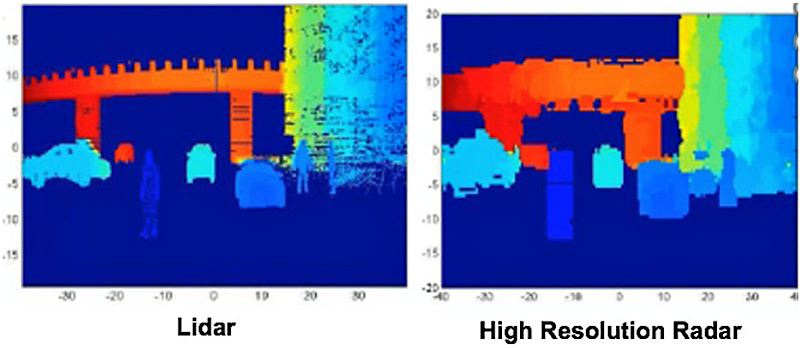
\includegraphics[width=\textwidth]{lidar-radar.png}
  \captionbelow[Vergleich Lidar und Radar Umgebungsscan. Quelle: \fullcite{lidar-radar})]{Vergleich Lidar und Radar Umgebungsscan (\cite{lidar-radar})}
  \label{lidar-radar}
\end{figure}

In den Fahrzeugen von Waymo, einem Tochterkonzern von Google's Mutterkonzern Alphabet, sind drei \acs{Lidar}-Scanner verbaut. Dazu gehören ein Kurzstrecken-\acs{Lidar} für den unmittelbaren Bereich um das Fahrzeug, ein Langstrecken-\acs{Lidar}, der auch aus mehreren hundert Metern Entfernung und voller Geschwindigkeit feine Signale, wie Handbewegungen, erkennen kann sowie einem hoch auflösenden \acs{Lidar}, welcher Millionen Laserimpulse aussenden kann, um ein detailliertes Bild der Umwelt zu erzeugen. \vgl{waymo} In autonomen Fahrzeugen wird \acs{Lidar} hauptsächlich für zwei Aufgaben eingesetzt:
\begin{enumerate}
  \item{Erkennung und Bestimmung von Objekten um das Fahrzeug}
  \item{Präzise Positionsbestimmung innerhalb der Fahrspur}
\end{enumerate}
\vgl{Surden}

Um das Fahrzeug präzise lokalisieren zu können, scannen \acs{Lidar}-Sensoren Straßenmarkierungen, indem sie die Straßenoberfläche auf unterschiedliche Reflexionsvermögen (aufgrund weißer Markierungen) untersuchen und speichern die Daten in einer Datei namens \acs{BLMR} (\acl{BLMR}). In der \acs{BLMR} werden stets die Leit- und Randliniendaten der letzten \SI{240}{\meter} gespeichert, diese werden laufend mit den zuvor erstellten annotierten digitalen Karten (siehe \ref{maps}) abgeglichen, wodurch der Standort bestimmt werden kann. \vgl{self-localization}

Sind keine Straßenmarkierungen vorhanden, können sich die Sensoren automatisch an anderen markanten Punkten wie Straßenschildern, Ampelanlagen, Gebäuden oder Bäumen, orientieren. Wichtig ist nur, dass es sich bei den Objekten um Dinge handelt, deren Standort sich nicht ändert und die eindeutig für \acs{Lidar}-Sensoren erkennbar sind.

\subsection*{Nachteile von Lidar}

Trotz der Vorteile wie der hohen Genauigkeit oder auch großen Reichweite haben auch \acs{Lidar}-Scanner Nachteile. Einer davon ist der Preis, besonders Geräte für große Distanzen sind teuer, da hierfür Laser mit \SI{1550}{\nano\meter} Wellenlänge benötigt werden, um für Menschen nicht schädlich zu sein. Um solche Laser wiederum empfangen zu können, sind Empfänger aus \ac{InGaAs} notwendig, da Siliziumempfänger, welche um ein Vielfaches günstiger als \ac{InGaAs} sind, keine Laserstrahlen mit \SI{1550}{\nano\meter} erkennen können. \vgl{wired} Durch jahrelange Entwicklung und ständig steigenden Produktionszahlen hat es Waymo mittlerweile geschafft, die Kosten für einen \acs{Lidar}-Scanner von \$\,\num{75000} um 90\,\% auf \$\,\num{7500} zu reduzieren. \vgl{waymo-medium}

Ein weiterer Nachteil ist die Abhängigkeit von gutem Wetter. Schnee, Regen oder Nebel reflektieren das Licht, was zur Folge hat, dass das Fahrzeug fälschlicherweise Hindernisse erkennt, welche in Wirklichkeit nur Regentropfen oder Schneeflocken sind. Dieser Bereich unterliegt aktuell noch weiteren Forschungen, Ford hat jedoch schon einen Algorithmus entwickelt, der dieses Problem beheben soll. Dabei werden die empfangenen Laserstrahlen genau auf ihre Eigenschaft untersucht, etwa ob sich ein Objekt zweimal an der selben Stelle befindet, was bei Regentropfen nicht der Fall ist. \vgl{ford-qz}
